% universal settings
\documentclass[12pt,twoside,onecolumn,openany,extrafontsizes,dvipsnames]{memoir}

\usepackage[utf8]{inputenc}
\usepackage[T1]{fontenc}
\usepackage{graphicx}

\usepackage{subcaption}
\usepackage{amsmath}
\usepackage{color}
\usepackage{listings}
\usepackage{xcolor}



\definecolor{codegreen}{rgb}{0,0.6,0}
\definecolor{codegray}{rgb}{0.5,0.5,0.5}
\definecolor{codepurple}{rgb}{0.58,0,0.82}
\definecolor{backcolour}{rgb}{0.95,0.95,0.92}

\lstdefinestyle{python_style}{
    backgroundcolor=\color{backcolour},   
    commentstyle=\color{codegreen},
    keywordstyle=\color{magenta},
    numberstyle=\tiny\color{codegray},
    stringstyle=\color{codepurple},
    basicstyle=\ttfamily\tiny,
    language=Python,
    numbers=left,
    stepnumber=1,
    numbersep=10pt,
    tabsize=4,
    showspaces=false,
    showstringspaces=false
}

\lstset{style=python_style}



%%%%%%%%%% BOOK INFORMATION %%%%%%%%%%
\title{Hands on Algorithms for robotics}
\author{Michal Chovanec, PhD.}
\date{\today}


\begin{document}
\maketitle


\chapter{Hardware description}
%\section{block diagram}


    \newpage
    \begin{figure}[h]
        \begin{subfigure}{.5\textwidth}
            \centering
            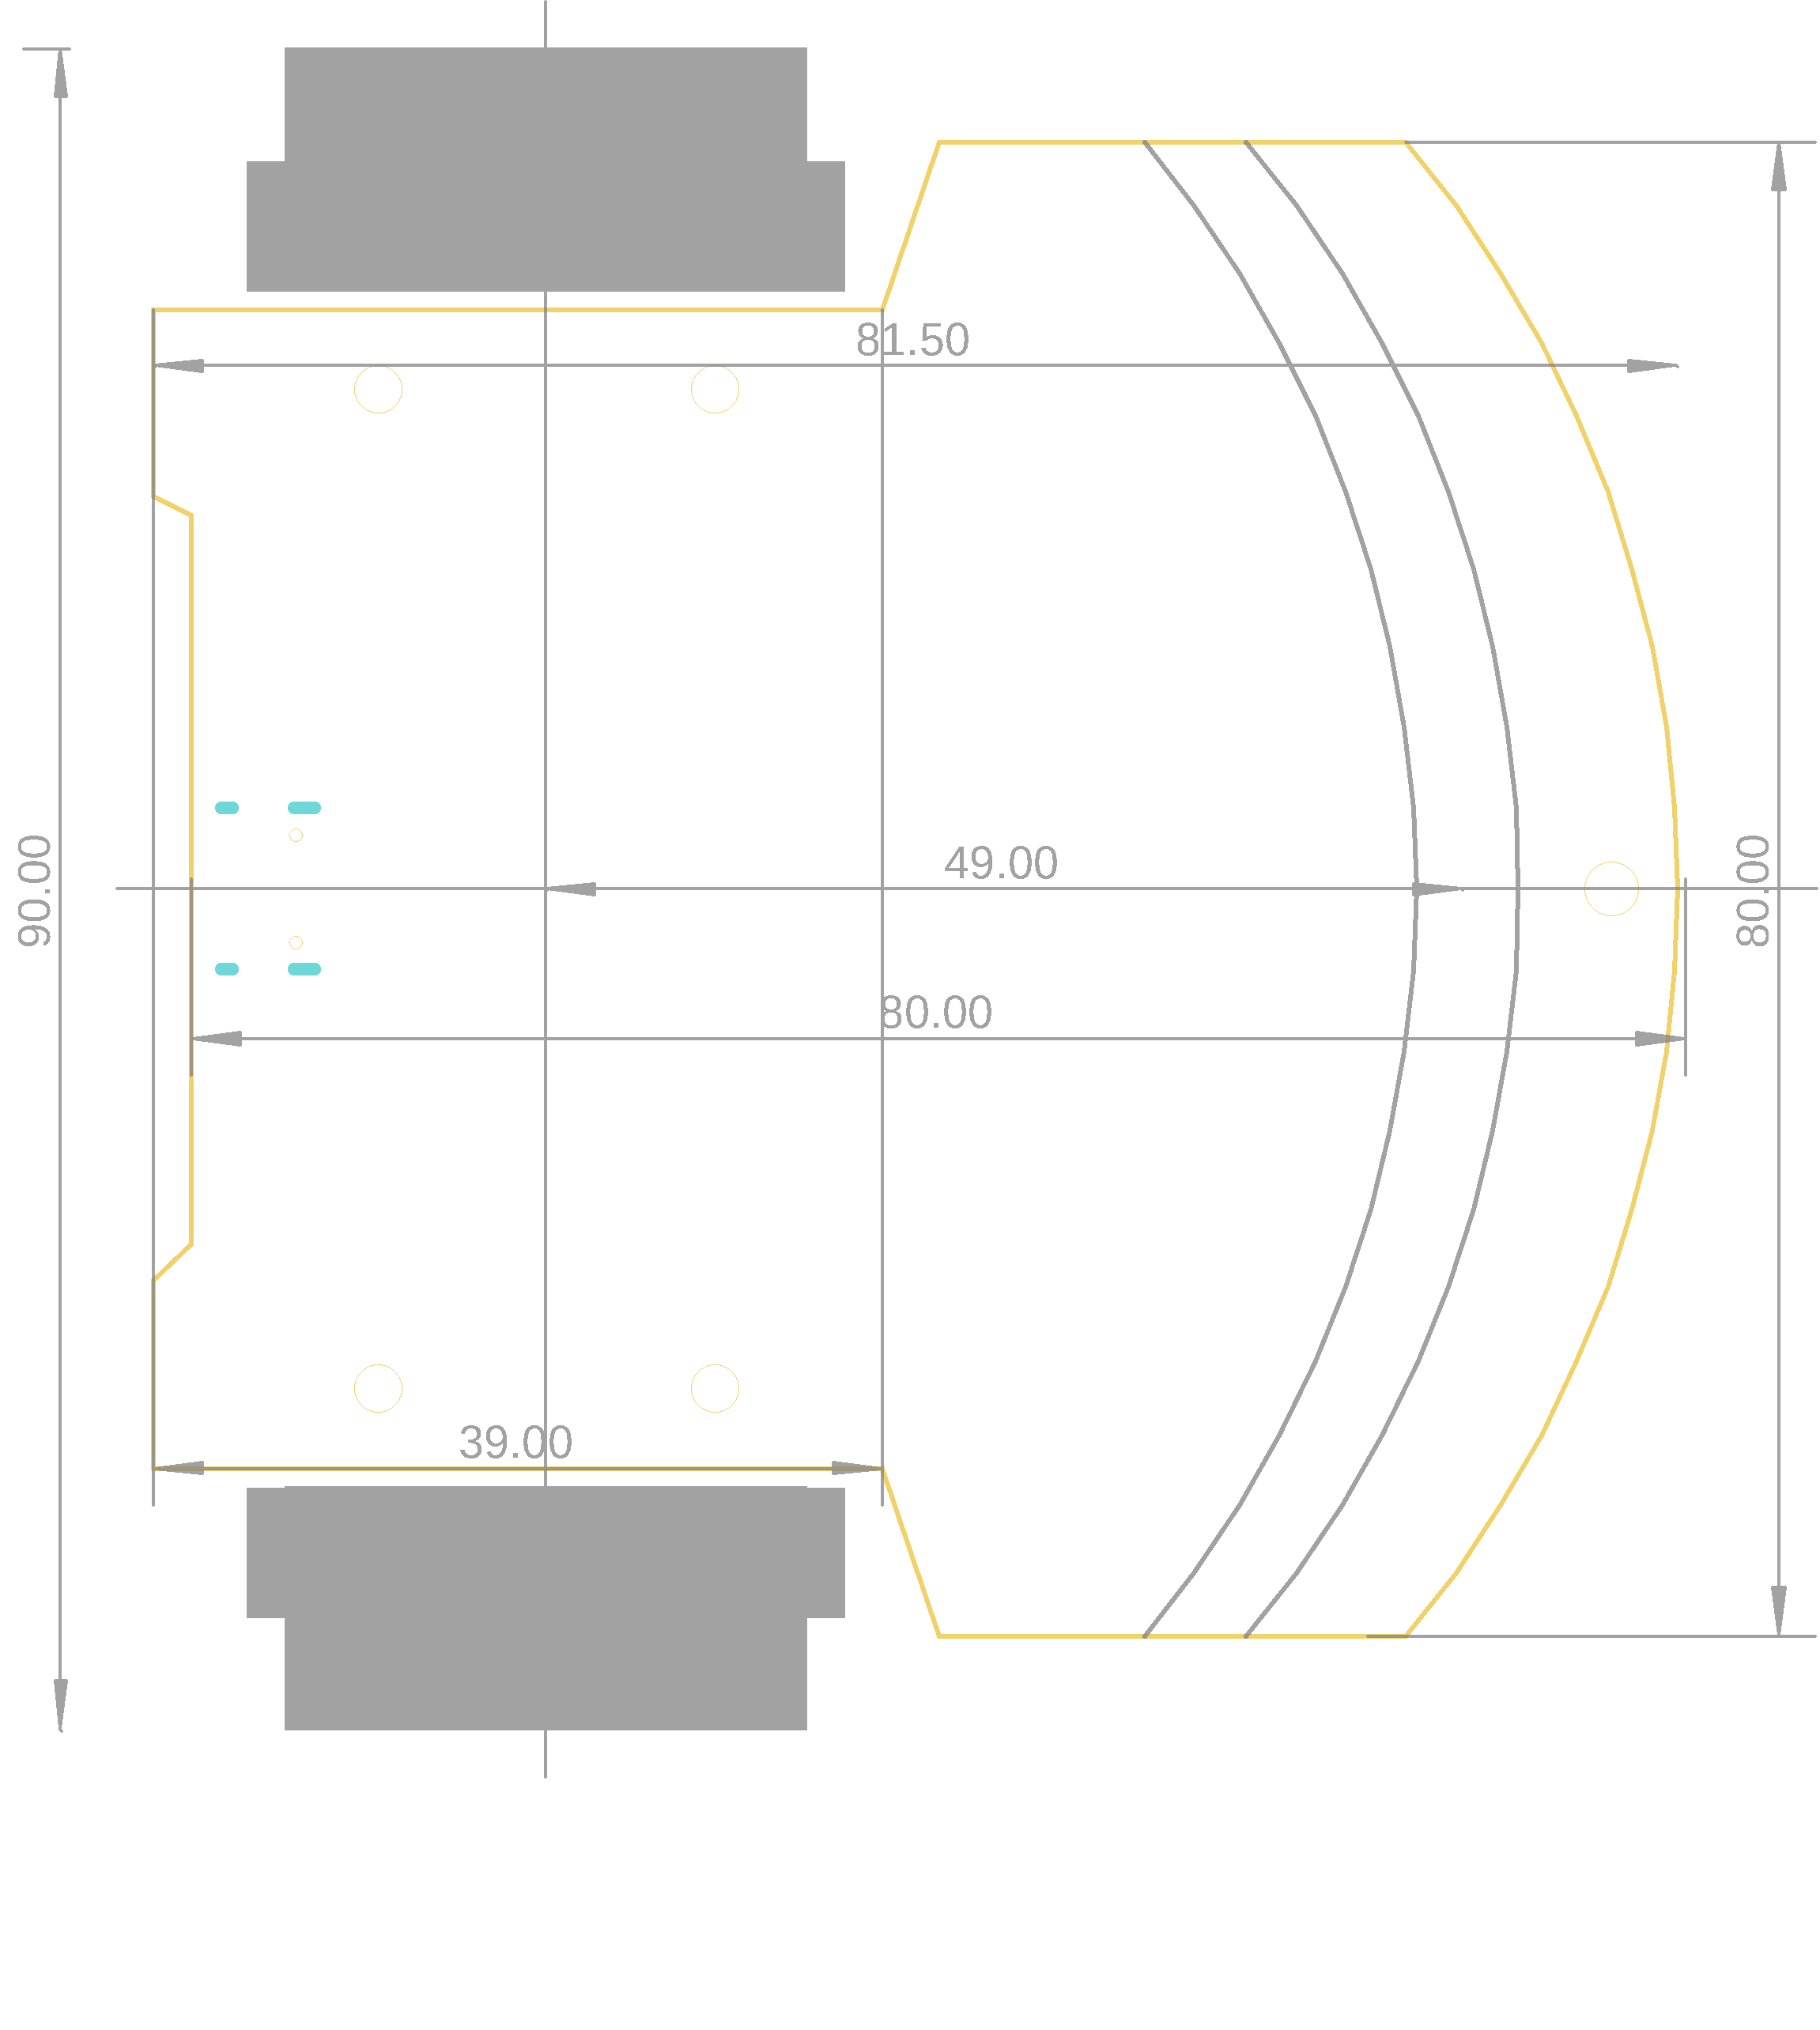
\includegraphics[scale=0.35]{../images/robot/board_dims_a.png}
            \caption{mechanical dimensions}
            \label{fig:mechanical_dimensions}
        \end{subfigure}%
        \begin{subfigure}{.5\textwidth}
            \centering
            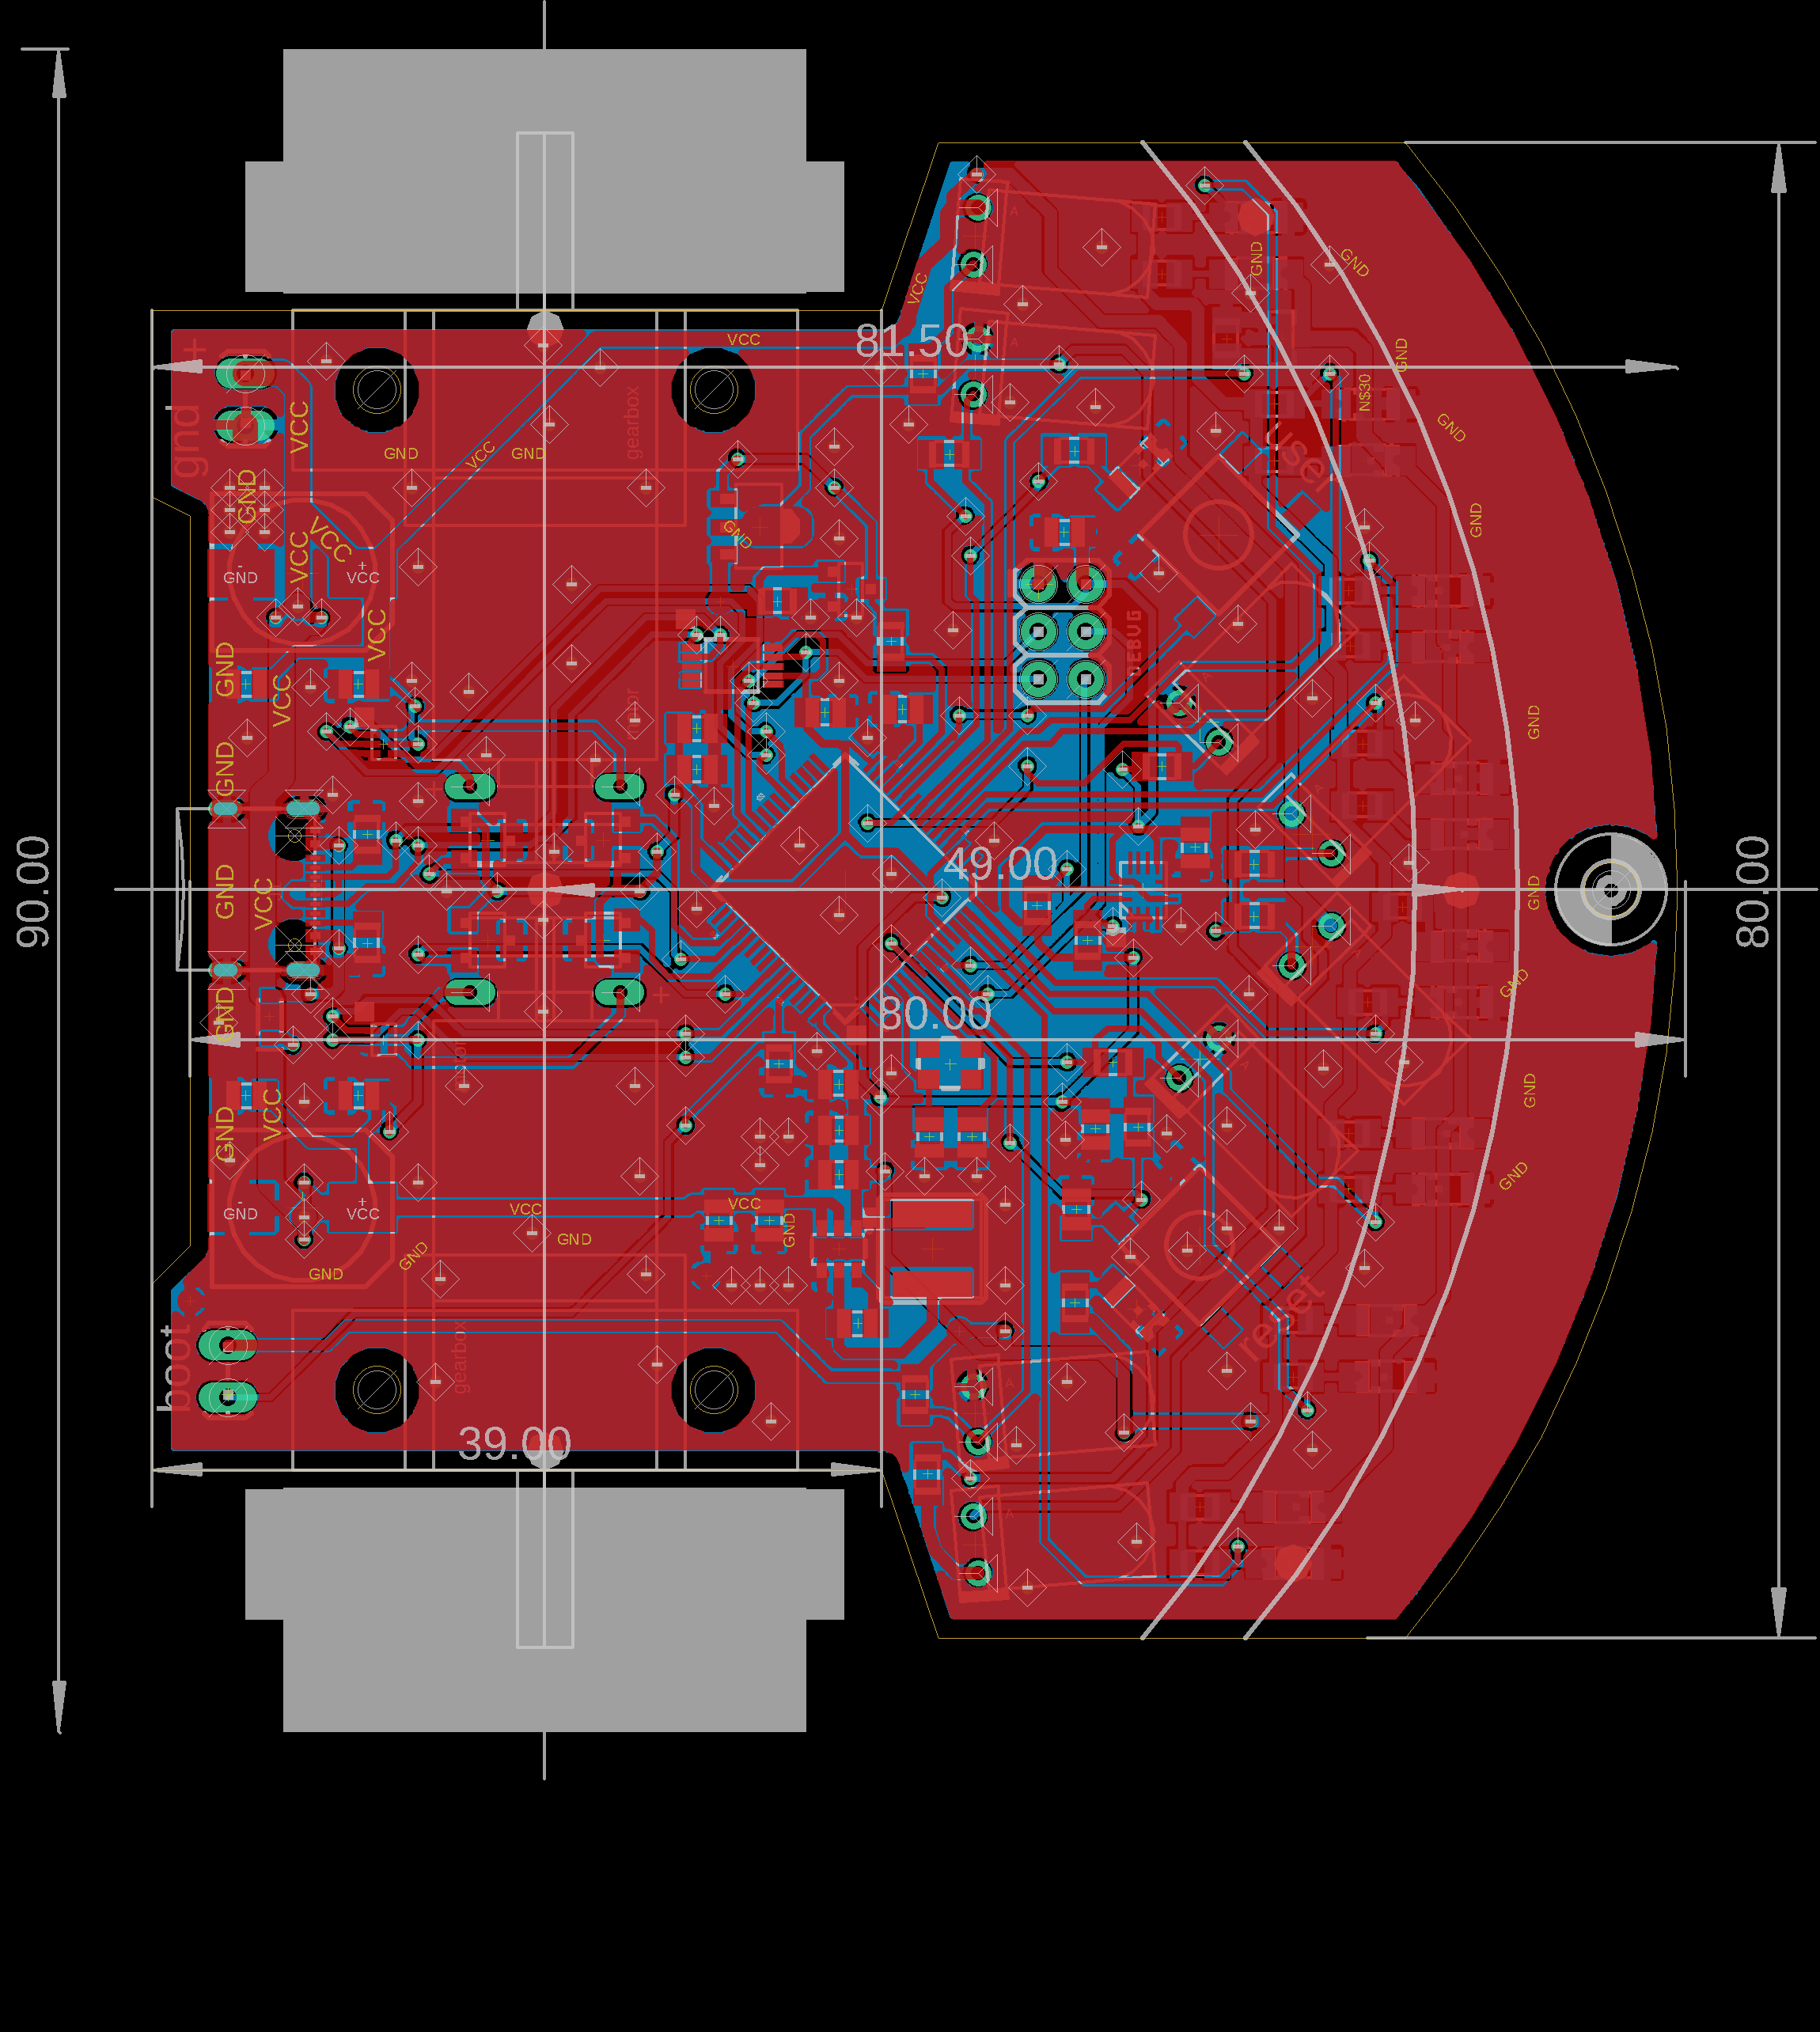
\includegraphics[scale=0.35]{../images/robot/board_all.png}
            \caption{overall PCB layout}
            \label{fig:overall_PCB_layout}
        \end{subfigure}


        \caption{Robot PCB}
    \end{figure}

    \begin{figure}[!b]
        \centering
        \includegraphics[scale=0.05]{../images/robot/robot_01.jpg}
        \caption{Robot photo}
        \label{fig:robot_photo}
    \end{figure}

    \newpage
    \begin{figure}[h]
        \centering
        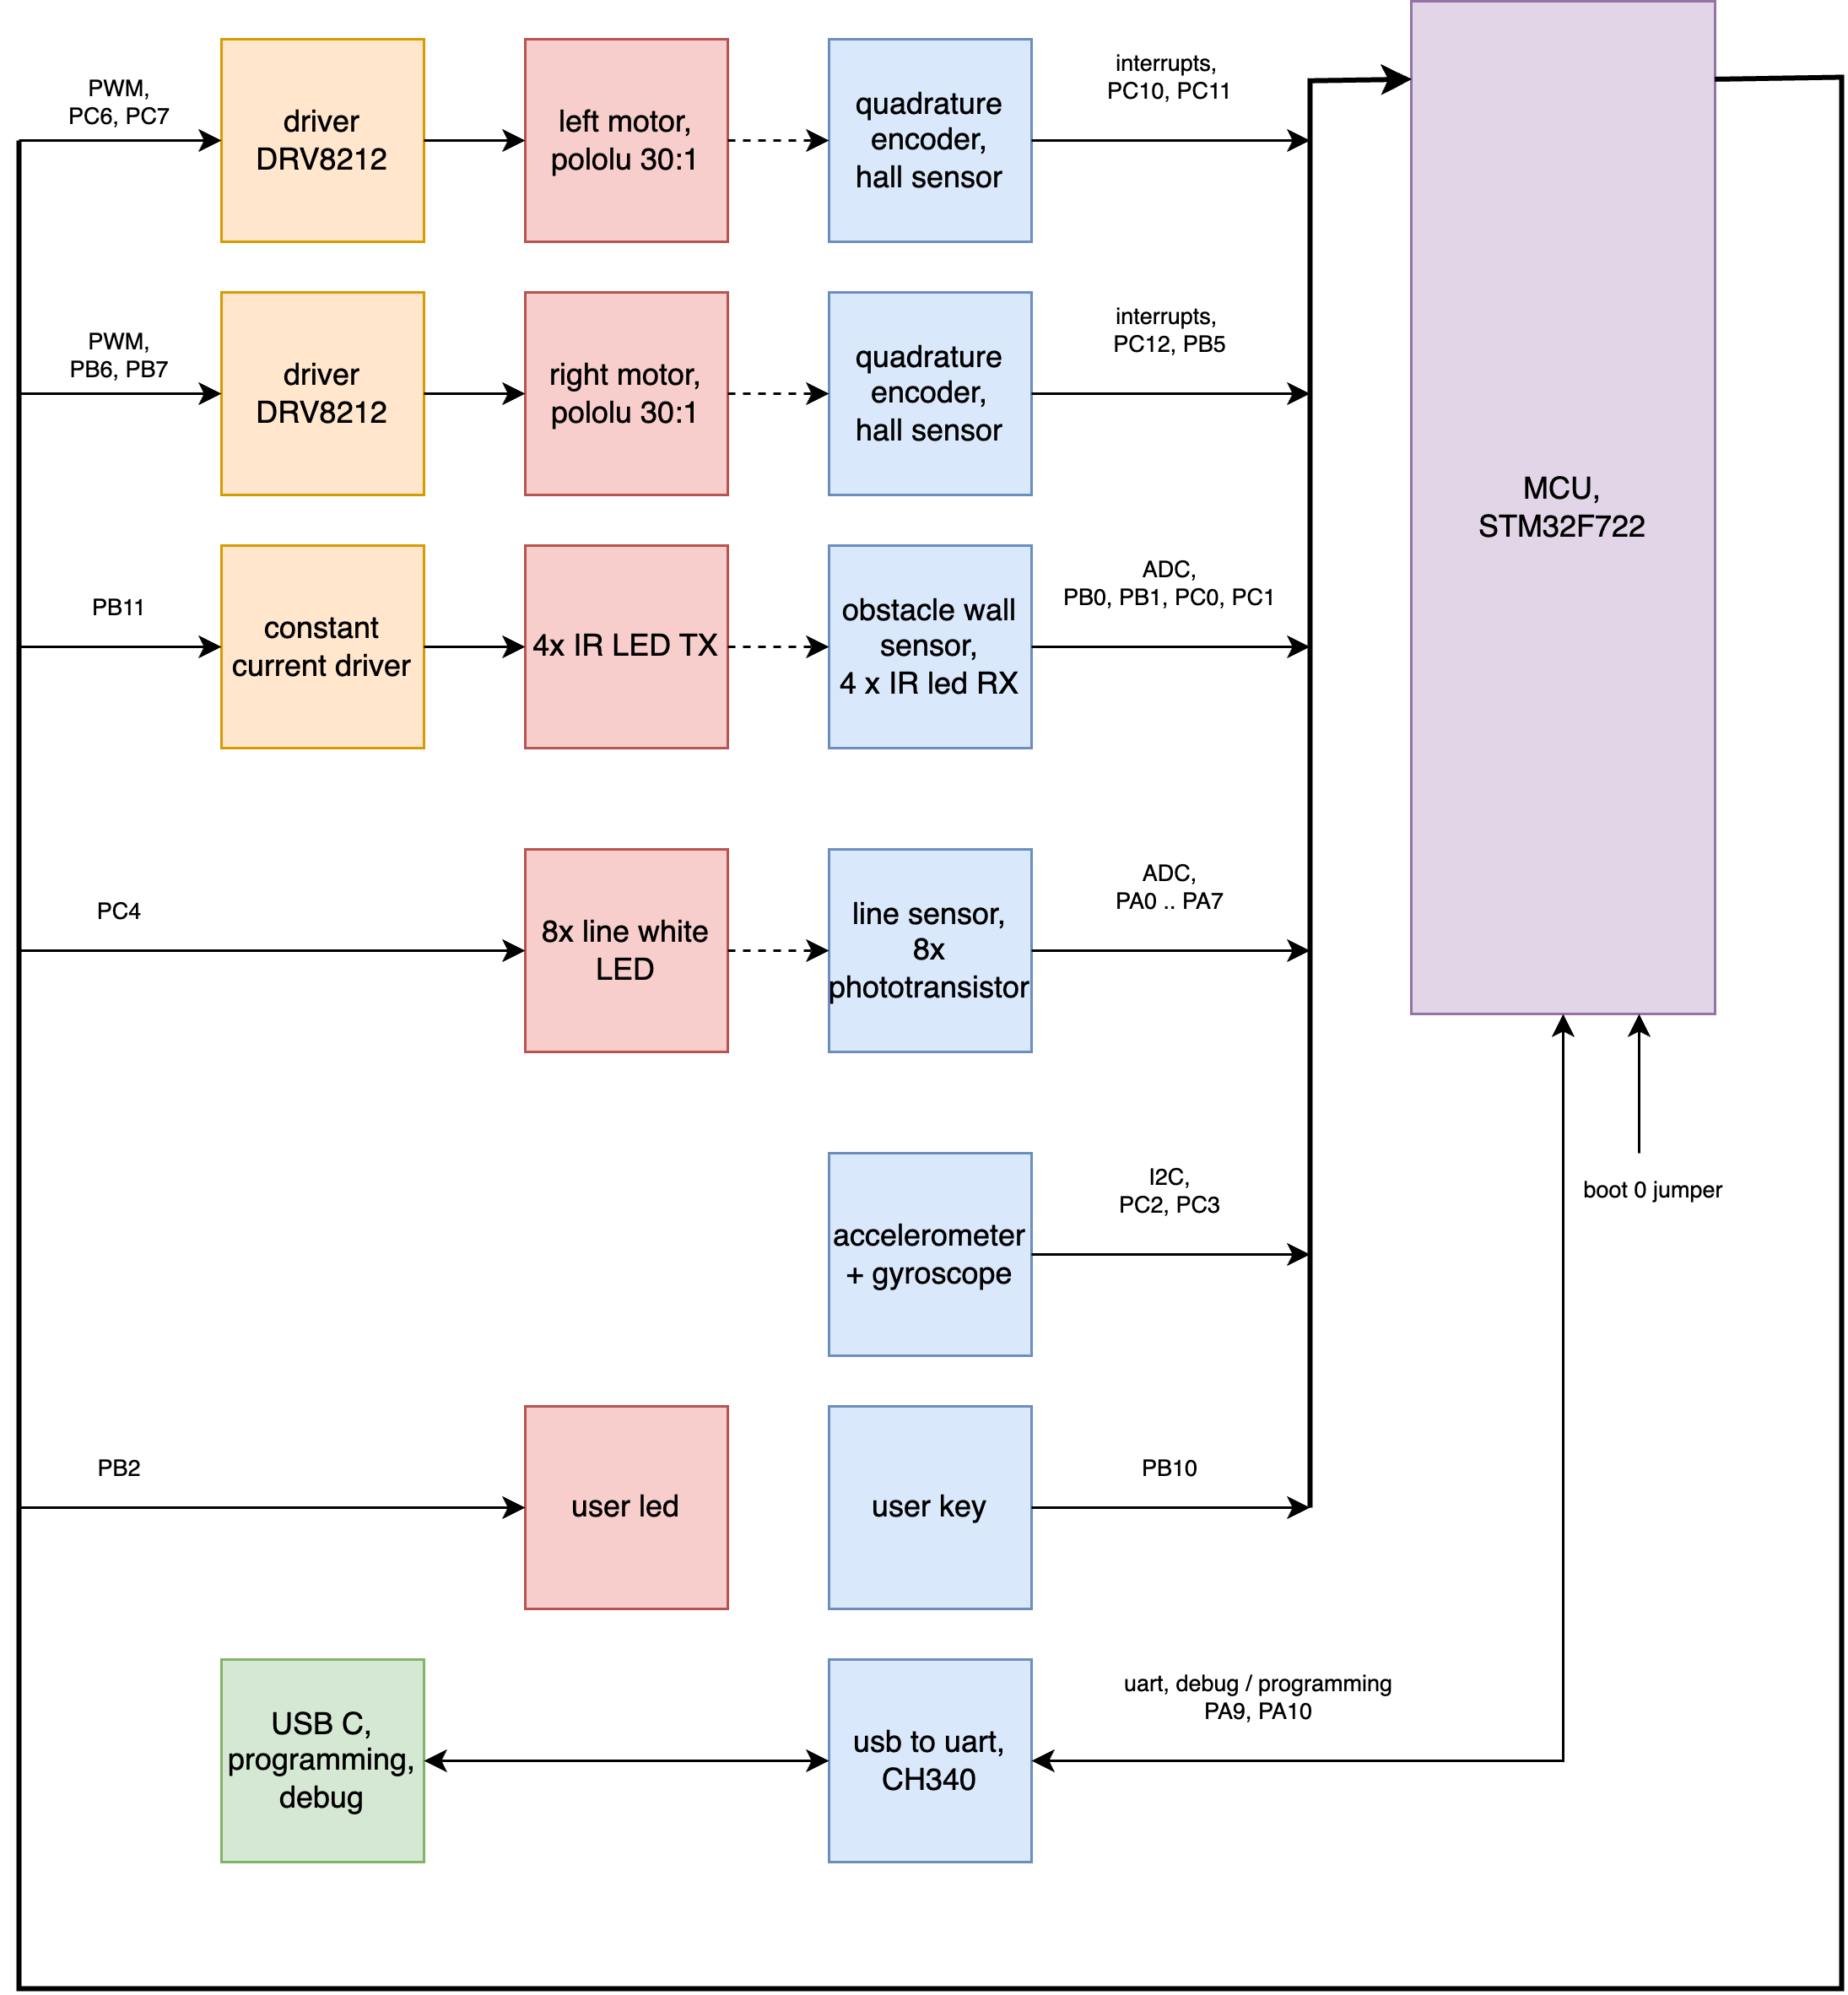
\includegraphics[scale=0.8]{../diagrams/sw/sw-block_dc.png}
        \caption{block diagram of DC motor version}
    \end{figure}

    \newpage
    \begin{figure}[h]
        \centering
        \includegraphics[scale=0.28]{../images/robot/schem_gs.png}
        \caption{schematic diagram of DC motor version}
    \end{figure}

    \newpage

        \begin{table}[h!]
            \centering
                \begin{tabular}{||c c c c c||} 
                \hline
                pin number & pin name & function & peripheral & AF number \\
                \hline\hline
                    14 & PA0 & line sensor ADC0, right & ADC1 & analog in \\ 
                    15 & PA1 & line sensor ADC1 & ADC1 & analog in \\ 
                    16 & PA2 & line sensor ADC2 & ADC1 & analog in \\ 
                    17 & PA3 & line sensor ADC3 & ADC1 & analog in \\ 
                    20 & PA4 & line sensor ADC4 & ADC1 & analog in \\ 
                    21 & PA5 & line sensor ADC5 & ADC1 & analog in \\ 
                    22 & PA6 & line sensor ADC6 & ADC1 & analog in \\ 
                    23 & PA7 & line sensor ADC7, left & ADC1 & analog in \\ 
                    & & & & \\
                    25 & PB0 & IR sensor ADC8, front left  & ADC1 & analog in \\ 
                    26 & PB1 & IR sensor ADC9, left & ADC1 & analog in \\ 
                    8 & PC0 & IR sensor ADC10, right & ADC1 & analog in \\ 
                    9 & PC1 & IR sensor ADC11, front right & ADC1 & analog in \\ 
                    & & & & \\
                    51 & PC10 & encoder left A  & GPIOC &  \\ 
                    52 & PC11 & encoder left B  & GPIOC &  \\ 
                    53 & PC12 & encoder right A  & GPIOC &  \\ 
                    57 & PB5  & encoder right B  & GPIOB &  \\ 
                    & & & & \\
                    37 & PC6 & PWM left A   & TIM3\_CH1 & AF2 \\     
                    38 & PC7 & PWM left B   & TIM3\_CH2 & AF2 \\ 
                    58 & PB6 & PWM right A  & TIM4\_CH1 & AF2 \\ 
                    59 & PB7 & PWM right B  & TIM4\_CH2 & AF2 \\ 
                    & & & & \\
                    10 & PC2 & IMU I2C, SDA & GPIOC &  \\ 
                    11 & PC3 & IMU I2C, SCL & GPIOC &  \\ 
                    & & & & \\
                    42 & PA9 & uart TX & UART1 & AF7 \\ 
                    43 & PA10 & uart RX & UART1 & AF7 \\ 
                    & & & & \\
                    27 & PB2 & user LED & GPIOB &  \\ 
                    28 & PB10 & user Key & GPIOB &  \\ 
                    29 & PB11 & IR LED control & GPIOB &  \\ 
                    24 & PC4 & line LED control & GPIOC &  \\ 
                    & & & & \\
                    7 & NRST & reset &  &  \\ 
                    60 & BOOT0 & firmware bootloader control &  &  \\ 
                \hline
                \end{tabular}
            \caption{pin mapping and function}
            \label{table:1}
        \end{table}

\newpage
\chapter{System identification}

    \section{State space models}

        System state is column vector, with $N$ rows
        \begin{align}
            x(n) &= \begin{bmatrix} x_{0}(n) \\ x_{1}(n) \\ ... \\ x_{N-1}(n) \end{bmatrix}
        \end{align}

        For single output system this vector contains single value, e.g. the motor velocity $\omega(n)$
        \begin{align}
            x(n) &= \begin{bmatrix} \omega(n) \end{bmatrix}
        \end{align}


        If we have 2nd order system, e.g. servo with inertia, the state will contain two 
        elements : 
        \begin{itemize}
            \item motor shaft velocity $\omega(n)$, measured in $rad/s$
            \item motor shaft angle $\theta(n)$, measured in $rad$
        \end{itemize}

        \begin{align}
            x(n) &= \begin{bmatrix} \omega(n) \\ \theta(n) \end{bmatrix}
        \end{align}

        More accurate servo model observes also motor current $i(n)$, which gives us three element state vector
        \begin{align}
            x(n) &= \begin{bmatrix} i(n) \\ \omega(n) \\ \theta(n) \end{bmatrix}
        \end{align}

        Robot moving in 2D plane have usualy state containing robot position $x'$, $y'$, and robot orientation $\theta$

        \begin{align}
            x(n) &= \begin{bmatrix} x'(n) \\ y'(n) \\ \theta(n) \end{bmatrix}
        \end{align}

        The number of rows in state vector $x(n)$ is called \textbf{system order}.

        The dynamical system is controlled with $M$ inputs, stacked in column input vector $u(n)$
        \begin{align}
            u(n) &= \begin{bmatrix} u_{0}(n) \\ u_{1}(n) \\ ... \\ u_{M-1}(n) \end{bmatrix}
        \end{align}

        The system with single input, e.g. motor with current control, input vector contains single value 
        \begin{align}
            u(n) &= \begin{bmatrix} i(n) \end{bmatrix}
        \end{align}

        Differential drive robot where are controlled two independent motors have two inputs 
        \begin{align}
            u(n) &= \begin{bmatrix} i_{left}(n) \\ i_{right}(n) \end{bmatrix}
        \end{align}

        Relation between control input $u(n)$, current state $x(n)$ and next state $x(n+1)$ can be 
        modeled using \textbf{linear state space model}
        
        \begin{align}
            x(n+1) &= Ax(n) + Bu(n)
        \end{align}

        \begin{figure}[!htb]
            \centering
            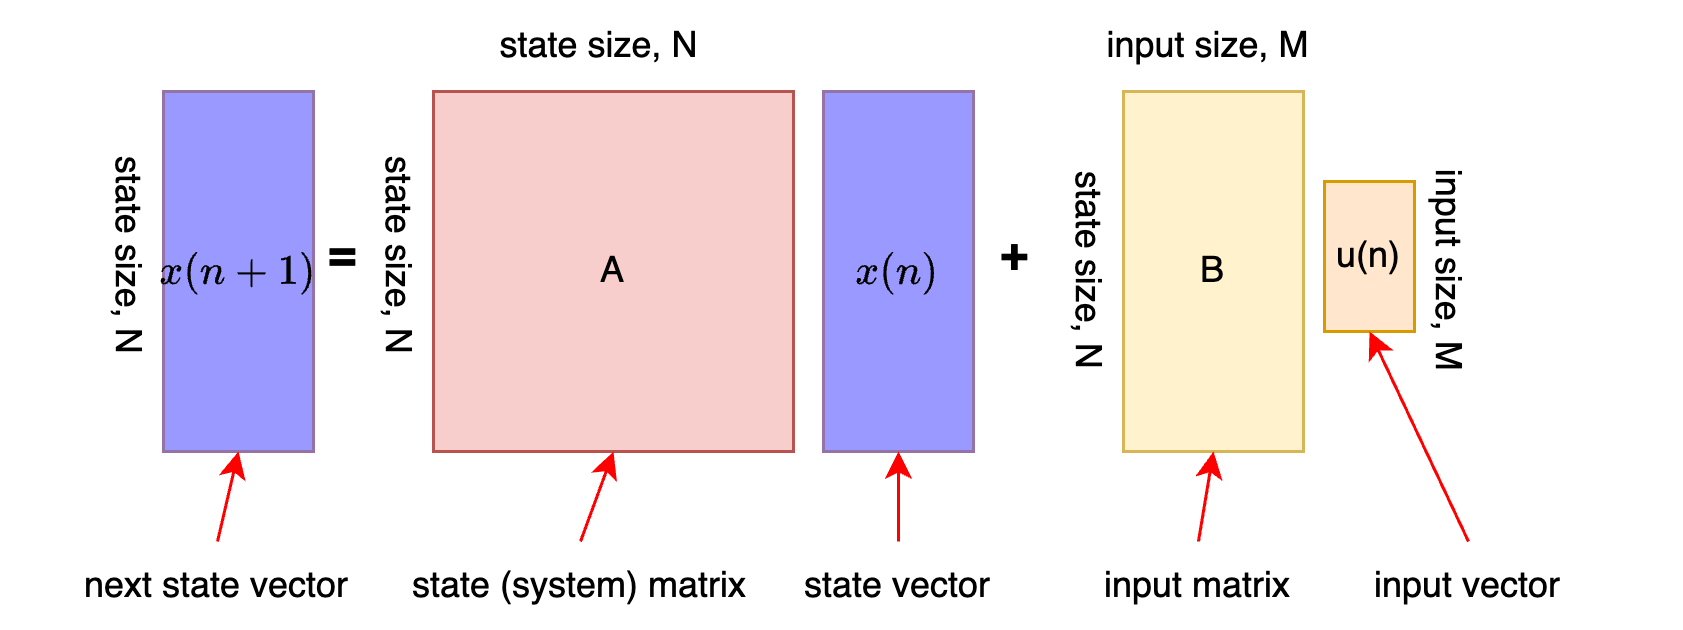
\includegraphics[scale=0.6]{../diagrams/control_generic/control_generic-discrete_dynamics.png}
            \caption{State space model matrices shapes}
            \label{fig:state_space_model_matrices_shapes}
        \end{figure}
        
        This model can capture dynamics of any linear system. Sometimes the state $x(n)$ can't be 
        meassured directly, and we observe only system output $y(n) = Cx(n)$. Where matrix $C$ have k-rows and n-columns.
        In our case we consider we have access to full state $x(n)$.
        There is of course the continuous form of state space model 

        \begin{align}
            \frac{dx}{dt} &= A^cx(t) + B^cu(t)
        \end{align}

        note : the martices $A^c$ and $B^c$ differs from discrete system matrices $A$ and $B$.
        They are related with bilinear transform as 
        
        \begin{align}
            S_a &= (I - \frac{\Delta T}{2}A^c)^{-1} \\
            S_b &= I + \frac{\Delta T}{2}A^c \\
            A &=  S_aS_b \\
            B &= S_a B^c \Delta T 
        \end{align}

        where $\Delta T$ is sampling period. This is mostly used discretisation, 
        from continuous (e.g. physical) model into discrete form.
        Following pythoncode convert continous system into discrete system. 
        If system contains output matrix $C$ discretisation doesn't effects its values.
       
        \begin{lstlisting}[style=python_style]
def c2d(a, b, c, dt):
    i = numpy.eye(a.shape[0])
    
    tmp_a = numpy.linalg.inv(i - (0.5*dt)*a)
    tmp_b = i + (0.5*dt)*a

    a_disc  = tmp_a@tmp_b
    b_disc  = (tmp_a*dt)@b

    return a_disc, b_disc, c
        \end{lstlisting}
       
        Process of system identification is finding matrices $A$, $B$ (and $C$). From this model 
        can be sythetised controller, or system able to plan multiple steps ahead.

    \section{First order identification}   
        Goal is to find parameters of DC motor. Motor velocity model, can be approximated as 1st linear order system. 
        Real system is of course non-linear. The photo of example system is on fig \ref{fig:wheel_drive_detail}.
        Control loop hardware consists of motor driver (H-driver, DRV8212), motor (Pololu HP 1:30 gear), and quadrature magnetic encoder (2x DRV5013),
        fig \ref{fig:motor_identification_process}

        \begin{figure}[!htb]
            \centering
            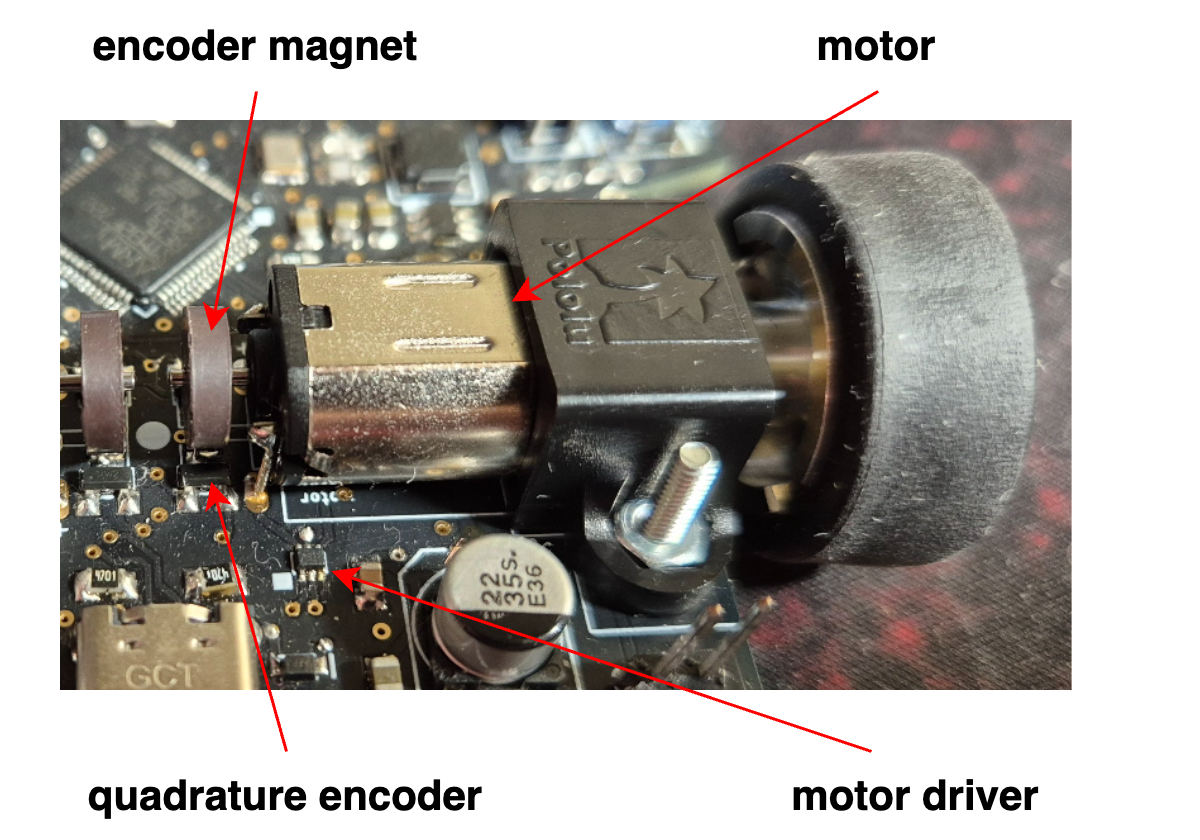
\includegraphics[scale=0.8]{../diagrams/control_generic/control_generic-motor_control_photo.png}
            \caption{Wheel drive hardware detail}
            \label{fig:wheel_drive_detail}
        \end{figure}

        \begin{figure}[!htb]
            \centering
            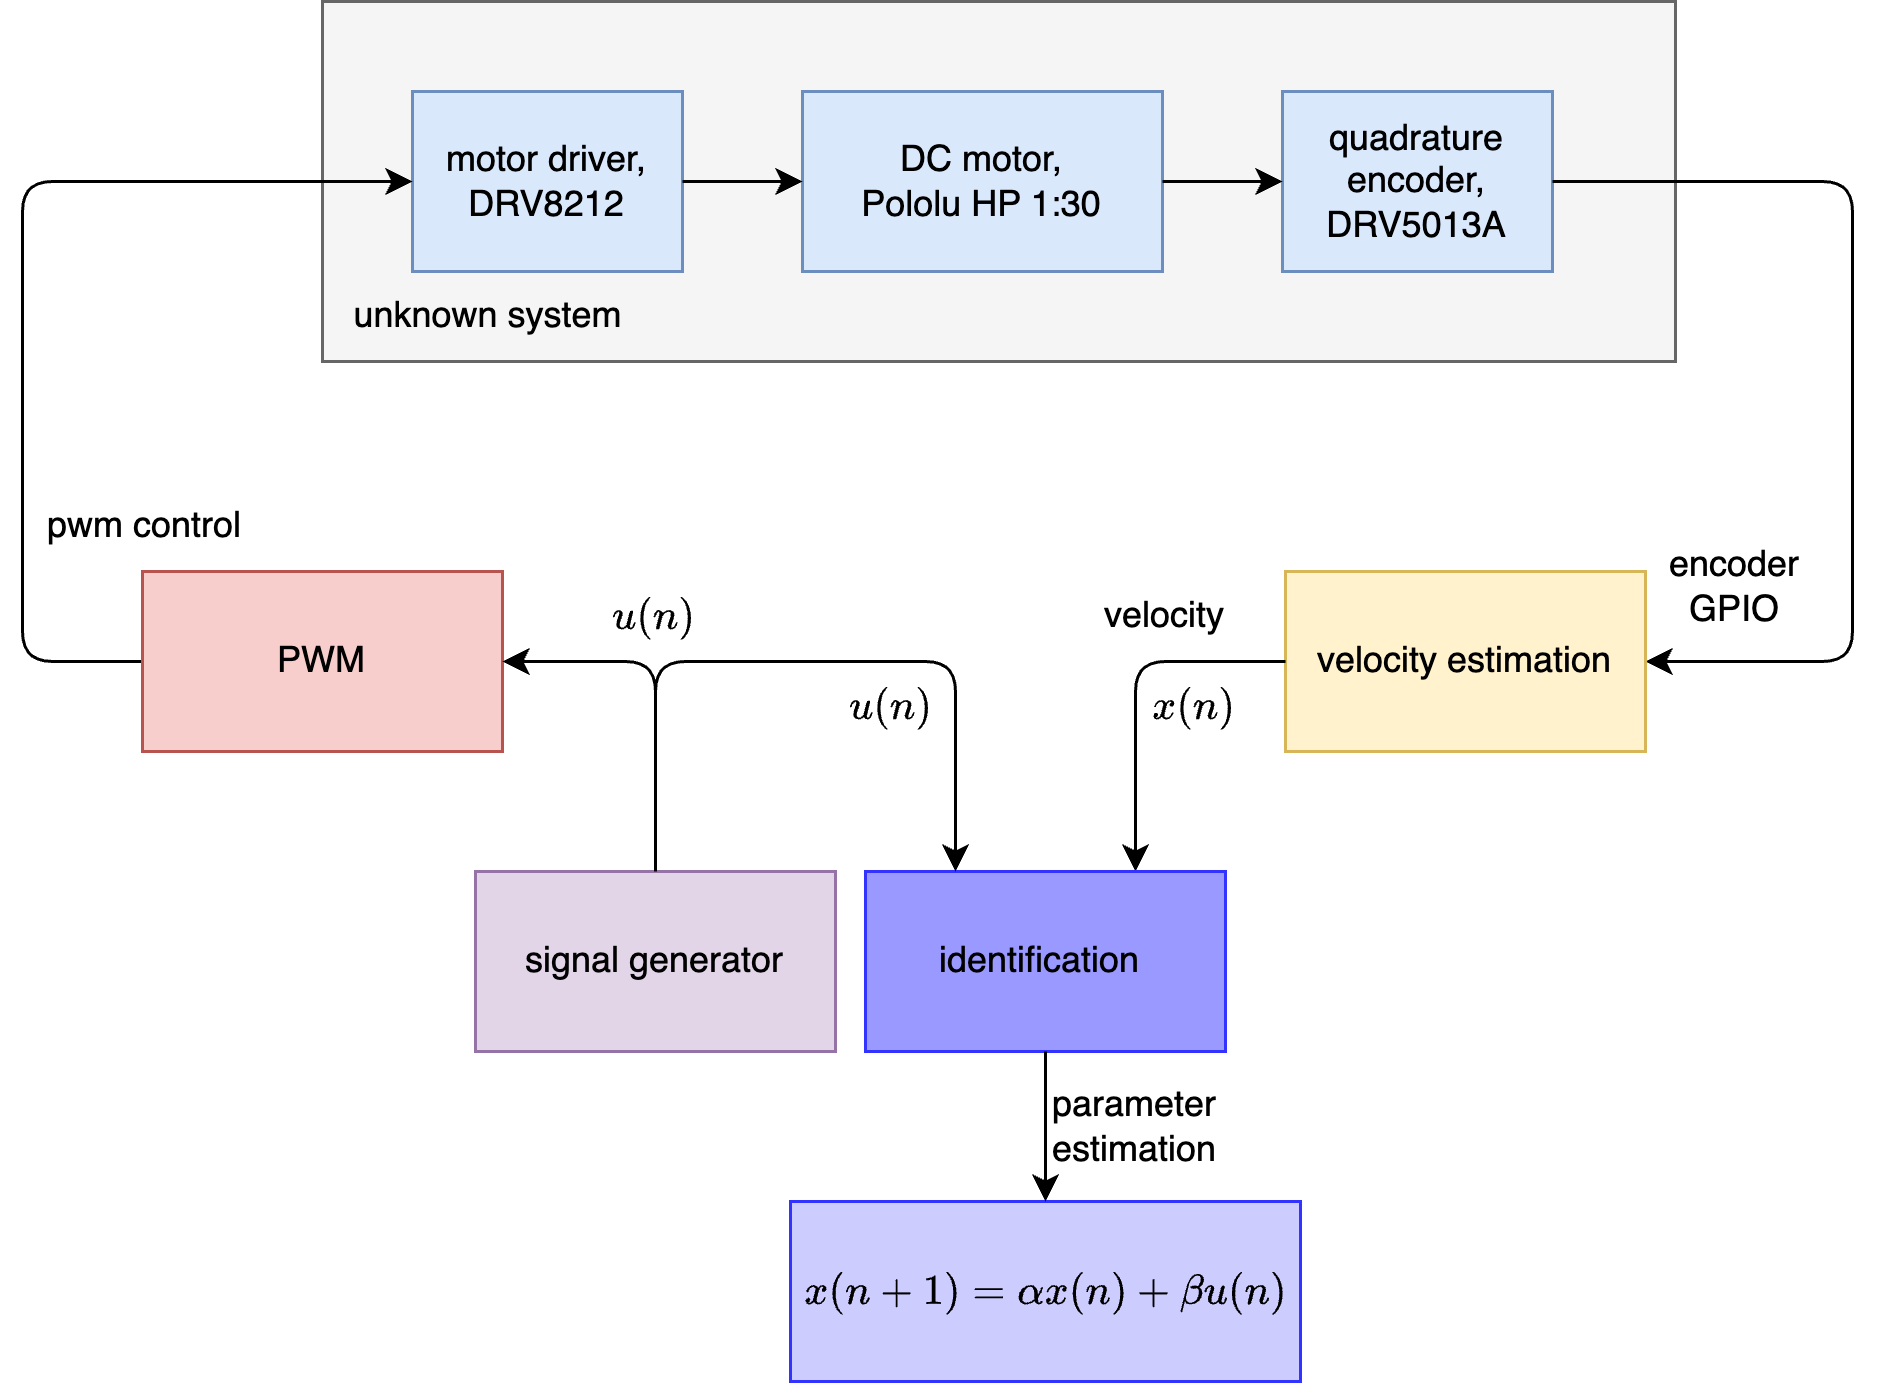
\includegraphics[scale=0.6]{../diagrams/identification/identification.png}
            \caption{Motor identification process}
            \label{fig:motor_identification_process}
        \end{figure}

        Input signal $u(n)$ can be generated arbitrarily. Mostly used is square wave, to capture
        high frequency dynamics. Algorithm is from observed motor velocity $x(n)$ and given input $u(n)$
        estimating model parameters.

        Before real motor testing, we focus on simulation example.
        Our simulated motor will have following parameters

        \begin{itemize}
            \item sampling frequency 4kHz, $\Delta T = 1/4000$
            \item maximum control input $u_{max} = 2$
            \item motor constant $k = 17$
            \item motor time constat $\tau = 29$ milliseconds
        \end{itemize}

        Motor state is single variable, angular velocity $\omega(t)$. Model have two parameters $\alpha$, $\beta$. 
        First order continuos model becomes

        \begin{align}
            \frac{d\omega(t)}{dt} &= \alpha \omega(t) + \beta u(t) \label{eq:first_order_system_a} \\
            \alpha &= -\frac{1}{\tau}  \label{eq:first_order_system_b} \\
            \beta &= \frac{k}{\tau}  \label{eq:first_order_system_c}
        \end{align}

        with given parameters $k$ and $\tau$ becomes $\alpha = -34.48$ and $\beta = 586.2$.

        Unit step response is obtained by setting $u(n) = 1$, and solving using any differential 
        equation solver. The simplest is Euler method, which works well for small $dt$ and low order 
        systems. Much accurate is commonly used Runge-Kutta 4 method.

        \begin{figure}[!htb]
            \centering
            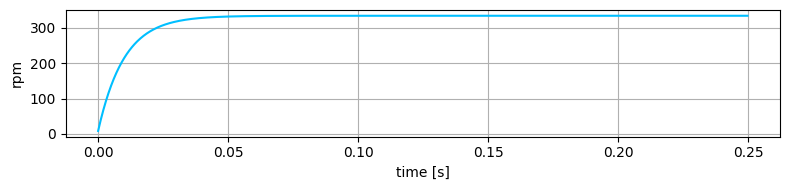
\includegraphics[scale=0.6]{../images/motor_control/motor_step_response.png}
            \caption{Motor step response}
            \label{fig:motor_step_response}
        \end{figure}

        Our goal is to generate input $u(t)$ and by observing system output $x(t)$ estimate parameters
        $k$ and $\tau$.

        We start with simplest identification method, which works only for 1st order non-oscilating systems.
        Method have two main steps
        \begin{enumerate}
            \item steady state value estimation
            \item time constant estimation
        \end{enumerate}

        \subsection{Steady state estimation}

            We drive motor on different input levels, e.g. ranging from 10\% ... 100\%. Observing steady 
            state velocity the motor constant $k$ can be estimated.

            \begin{figure}[!htb]
                \centering
                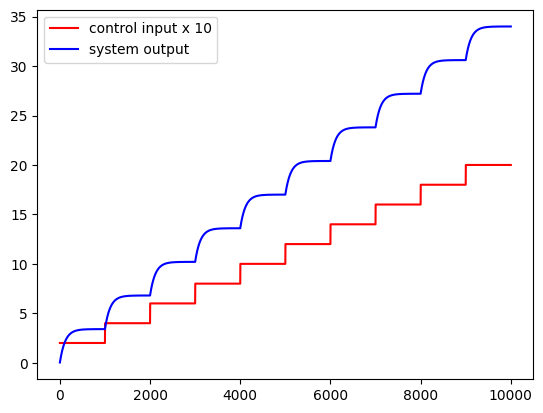
\includegraphics[scale=0.6]{../images/motor_control/motor_constant_estimation.png}
                \caption{Motor constant estimation}
                \label{fig:motor_constant_estimation}
            \end{figure}

            Algorithm for estimating motor constant :

            \begin{enumerate}
                \item choose constant motor input $u \in (0, u_{max} \rangle$
                \item run motor, and wait for velocity steady state
                \item measure velocity  
                \item estimate $\hat{k} = x/u$
                \item repeats to estimate average $\hat{k}$
            \end{enumerate}

            In following code we choose 10 different input levels. After setting, we wait 500steps
            to steady state, then we measure output velocity. Finally, we average results.

            \begin{lstlisting}[style=python_style]
# input levels
u_values = u_max*numpy.array([0.1, 0.2, 0.3, 0.4, 0.5, 0.6, 0.7, 0.8, 0.9, 1.0])

# reset dynamical system into zero state
ds.reset()

for j in range(len(u_values)):

    x_mean = []
    for i in range(1000):

        # convert scalar u to column vector
        u    = u_values[j]
        u    = numpy.array([[u]])
        
        # compute dynamical system one step
        x, _ = ds.forward_state(u)

        # after steady state, store x
        if i > 500:
            x_mean.append(x[0][0])

    x_mean = numpy.array(x_mean)
    x_mean = x_mean.mean()

    k_est = x_mean/u_values[j]

    print(u_values[j], k_est)

k_mean = k_est.mean()

# average k estimate
print("k_mean = ", k_mean)
            \end{lstlisting}

        In our example the resulted $\hat{k}$ is $16.995$, which very close to real value $17$.
        Accuracy depends on velocity estimation noise (encoder noise) and how many samples we average.
        
        \subsection{Time constant estimation}

            Second parameter is time constant $\tau$. Most textbooks uses measuring time at which system 
            reaches $63.2\%$ of $x_{max}$. Where $x_{max}$ is motor velocity on choosen $u$, a.k.a. steady 
            state velocity at $u$. This method suffers to noise, and precise timing. Here we presents 
            more accurate method, briging system into natural frequency resonance.
            Algorithm is as follow :
        
            \begin{enumerate}
                \item choose $u_{set}$, and set $u_{in} = u_{set}$
                \item repeat $n_{steps}$, each step duration is $\Delta T$
                    \begin{enumerate}
                        \item $if\ u_{in} > 0\ and\ x(n) > 0.632ku_{in}$ \\
                            increment $n_{HalfPeriods}$, and set $u_{in} = -u_{in}$
                        \item $else\ if\ u_{in} < 0\ and\ x(n) < 0.632ku_{in}$ \\
                            increment $n_{HalfPeriods}$, and set $u_{in} = -u_{in}$
                    \end{enumerate}
            \end{enumerate}

            The time constant $\hat{\tau}$ can be now estimated by 

            \begin{align}   
                \hat{\tau} = \frac{2}{\pi}\frac{n_{steps}}{n_{HalfPeriods}}{\Delta T}
            \end{align}

            Where $\Delta T$ is sampling period, ratio ${n_{steps}} : {n_{HalfPeriods}}$ is
            estimating system frequency. In core, this method is nothing more than  period 
            duration estimation. The resulted time plot is on fig.  \ref{fig:motor_time_constant_estimation}.
            Result for our simulated motor is $\hat{\tau} = 27.44[ms]$, which is good estimation of real value $29 [ms]$.

            \begin{figure}[!htb]
                \centering
                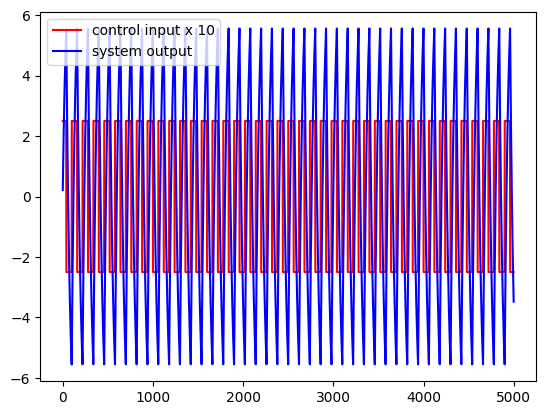
\includegraphics[scale=0.6]{../images/motor_control/motor_time_constant_estimation.png}
                \caption{Motor time constant estimation}
                \label{fig:motor_time_constant_estimation}
            \end{figure}
            
            Using equations \ref{eq:first_order_system_b} and \ref{eq:first_order_system_c} we can estimate $\hat{\alpha}$ and $\hat{\beta}$ as
            $\hat{\alpha} = -36.443$ and $\hat{\beta} = 619.372$

          

        \subsection{Real motor identification}
        TODO


\newpage
\chapter{Motor control}

    motor velocity controller

    \begin{figure}[!htb]
        \centering
        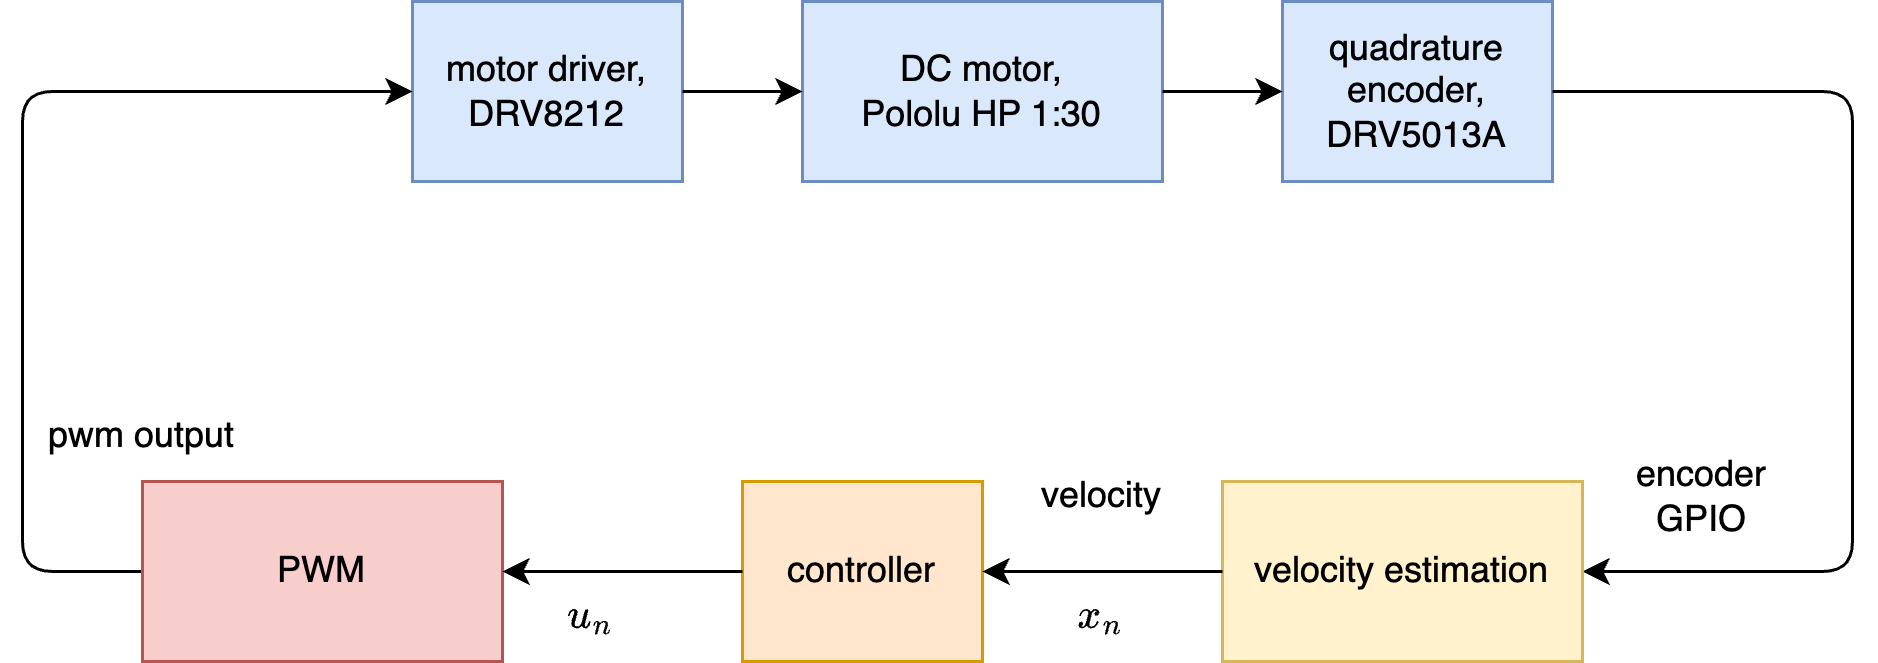
\includegraphics[scale=0.6]{../diagrams/control_generic/control_generic-motor_control.png}
        \caption{Velocity control overview}
        \label{fig:velocity_control_overview}
    \end{figure}


    \newpage
    \section{PID control}

        \begin{figure}[!htb]
            \centering
            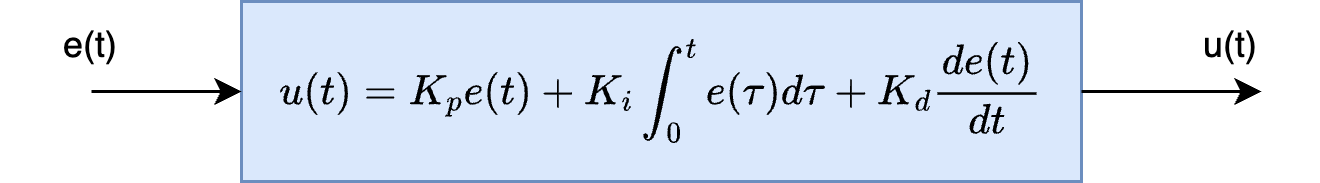
\includegraphics[scale=0.8]{../diagrams/control_generic/control_generic-pid.png}
            \caption{Textbook continuous PID controller}
            \label{fig:textbook_continuous_pid_controller}
        \end{figure}

        \begin{figure}[!htb]
            \centering
            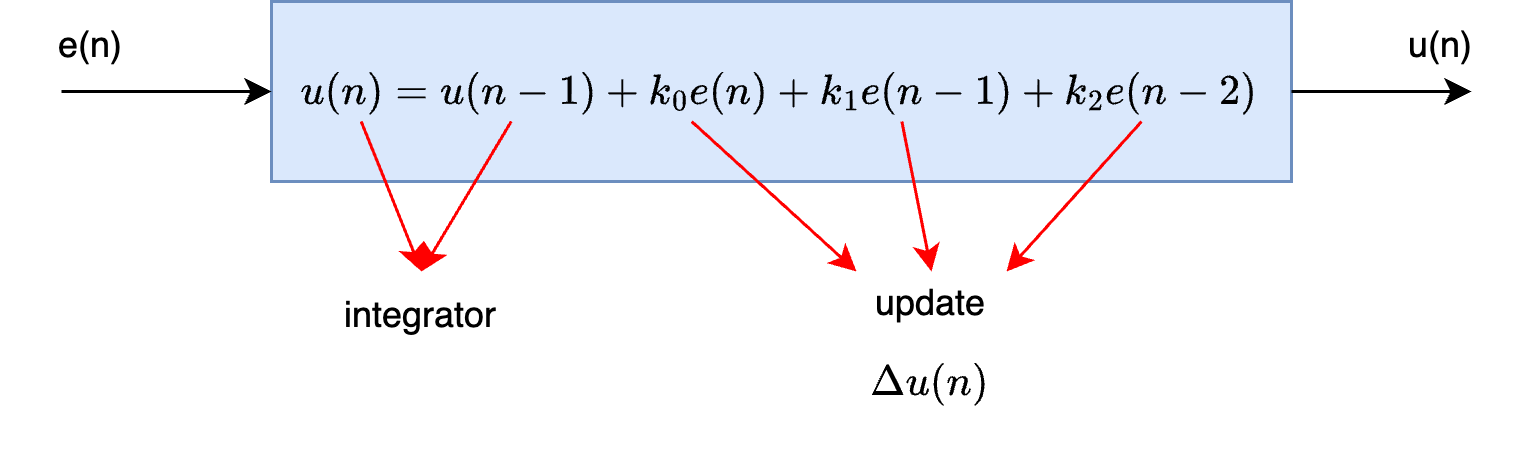
\includegraphics[scale=0.8]{../diagrams/control_generic/control_generic-pid_discrete.png}
            \caption{Discrete PID controller }
            \label{fig:discrete_pid_controller}
        \end{figure}

        
        \begin{align}
            k_0 &= K_p + K_i\Delta T + \frac{K_d}{\Delta T} \\
            k_1 &= -K_p - 2\frac{K_d}{\Delta T} \\
            k_2 &= \frac{K_d}{\Delta T}
        \end{align}

            \newpage
            \subsection{PID control - P only controller}

                \begin{itemize}
                    \item  target value : \textcolor{red}{\textbf { 1000rpm}}
                    \item  P-only control causes \textcolor{red}{\textbf {steady state error}}
                \end{itemize}
            
                \begin{align}
                    u(n+1) &= u(n-1) + k_pe(n) - k_pe(n-1) \\
                    k_p    &= 0.01
                \end{align}

                \begin{figure}[!htb]
                    \centering
                    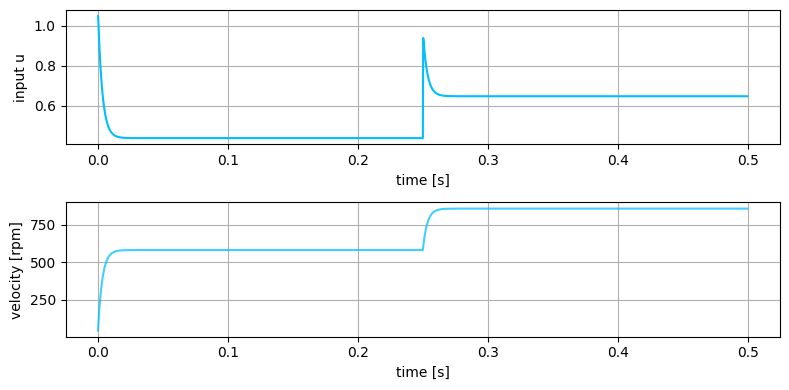
\includegraphics[scale=0.8]{../images/motor_control/pid_p_control.png}
                    \caption{P-only controller}
                    \label{fig:p_controller}
                \end{figure}

            \newpage
            \subsection{PID control - PI}
                
                too high I term 

                \begin{itemize}
                    \item  target value : \textcolor{red}{\textbf {1000rpm}}
                    \item  PI control \textcolor{red}{\textbf {removes steady state error}}
                    \item  too high I term causes \textcolor{red}{\textbf {oscilations and overshot}}
                \end{itemize}
            
              
                \begin{align}
                    u(n+1) &= u(n-1) + (k_p + k_i\Delta T) e(n) - k_pe(n-1) \\
                    k_p    &= 0.01 \\
                    k_i\Delta T    &= 0.005
                \end{align}
                
                
                \begin{figure}[!htb]
                    \centering
                    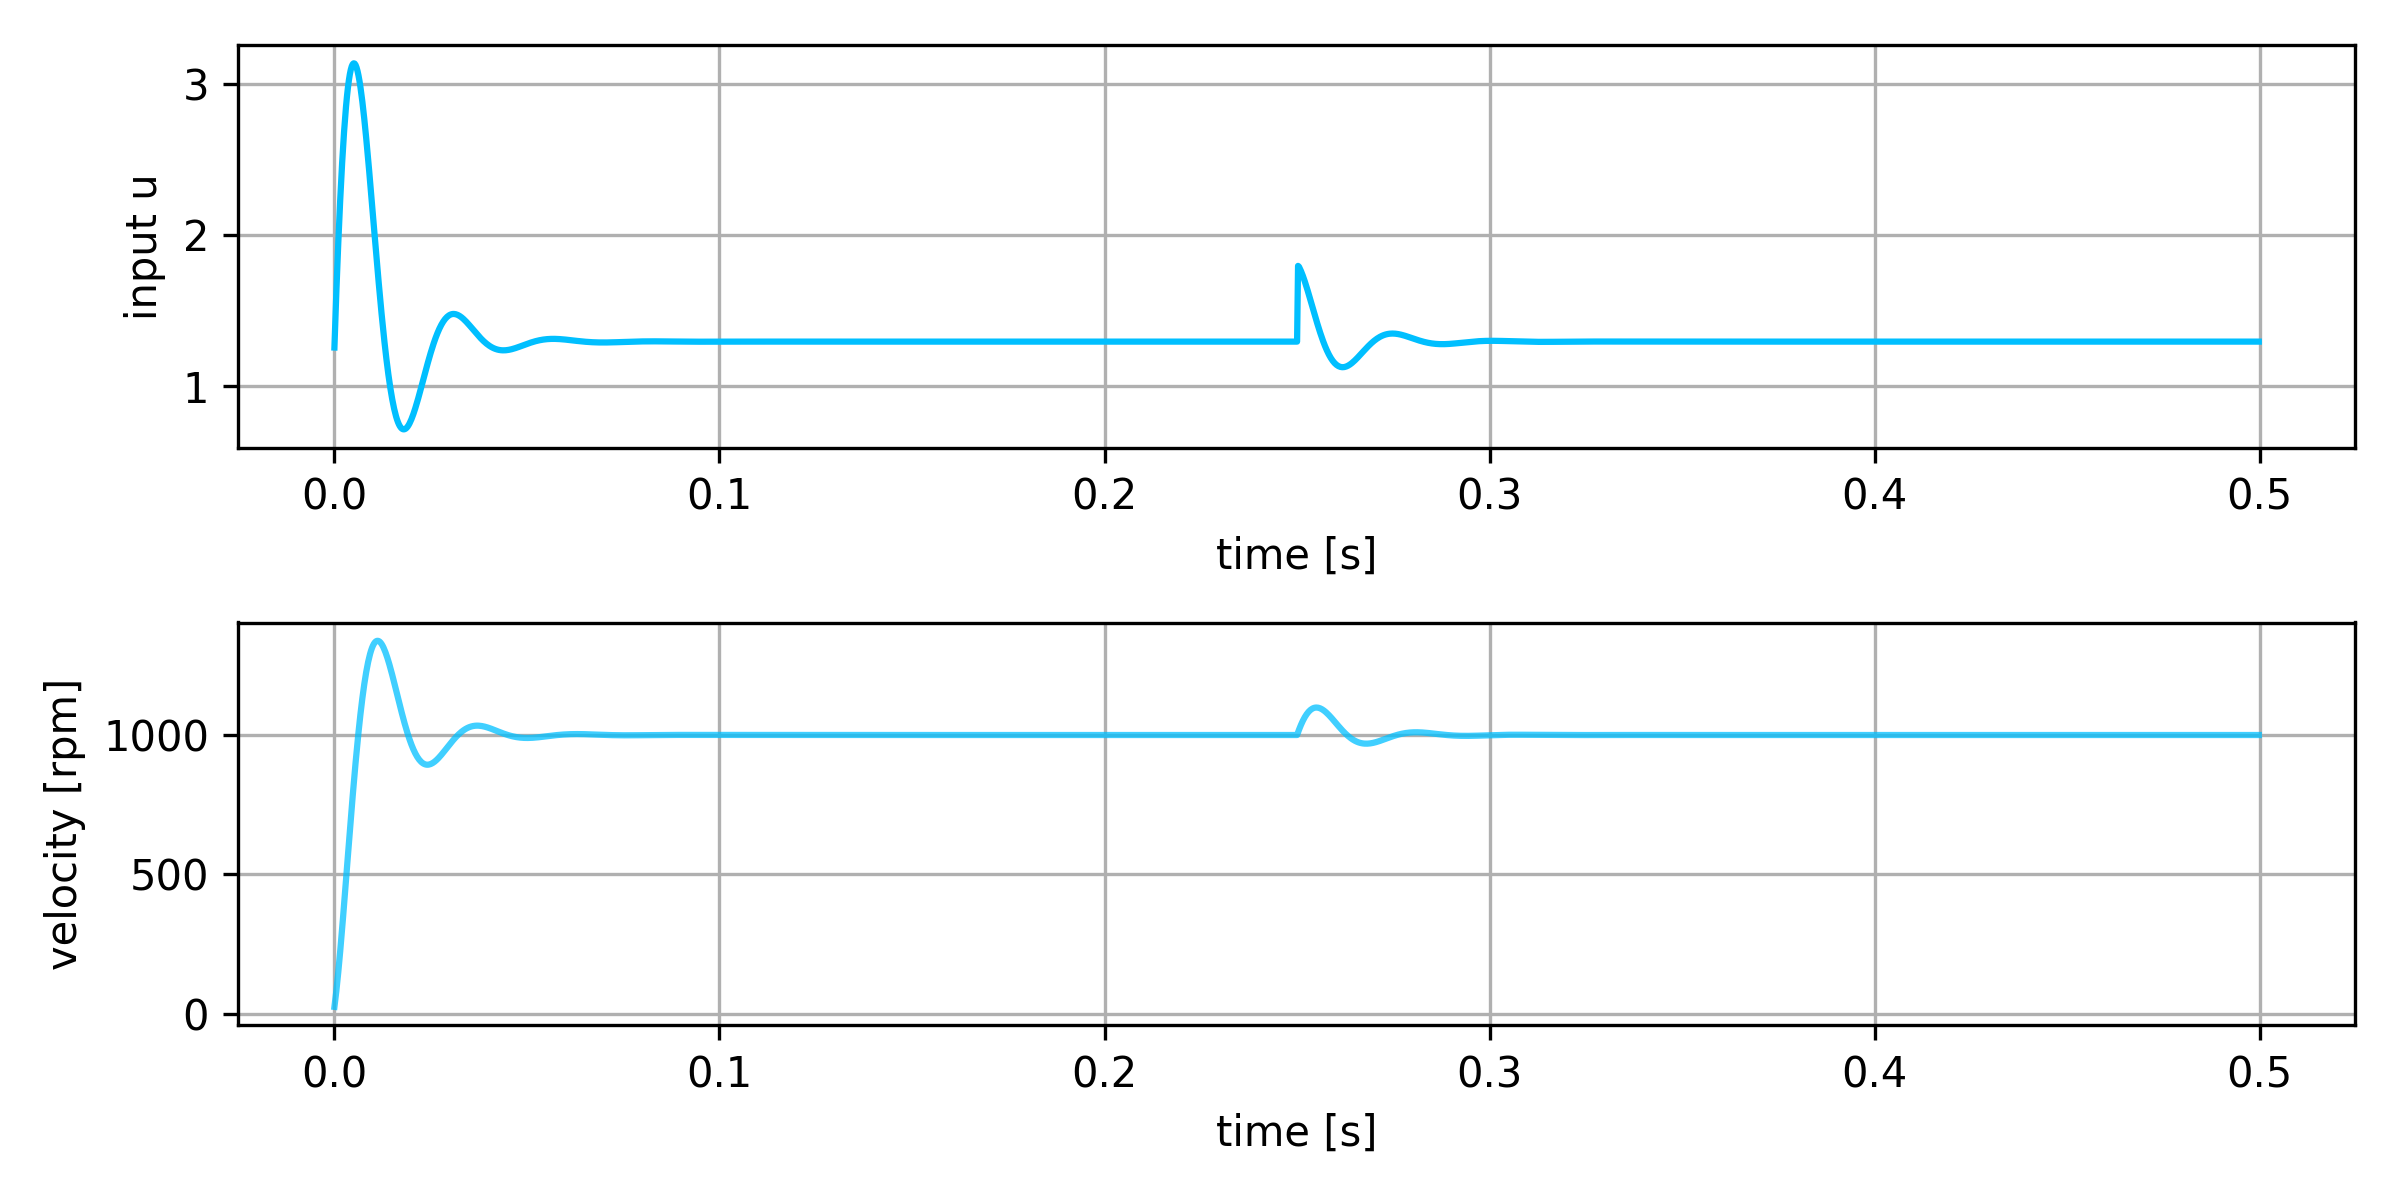
\includegraphics[scale=0.8]{../images/motor_control/pid_pi_control_0.png}
                    \caption{PI controller}
                    \label{fig:pi_controller}
                \end{figure}

                correct I term

                \begin{itemize}
                    \item  target value : \textcolor{red}{\textbf {1000rpm}}
                    \item  correct tunned PI controller for 1st order system
                    \item  \textcolor{red}{\textbf {no overshot, no steady state error}}
                \end{itemize}
                
                \begin{align}
                    u(n+1) &= u(n-1) + (k_p + k_i\Delta T) e(n) - k_pe(n-1) \\
                    k_p    &= 0.01 \\
                    k_i\Delta T    &= 0.0002
                \end{align}

                \begin{figure}[!htb]
                    \centering
                    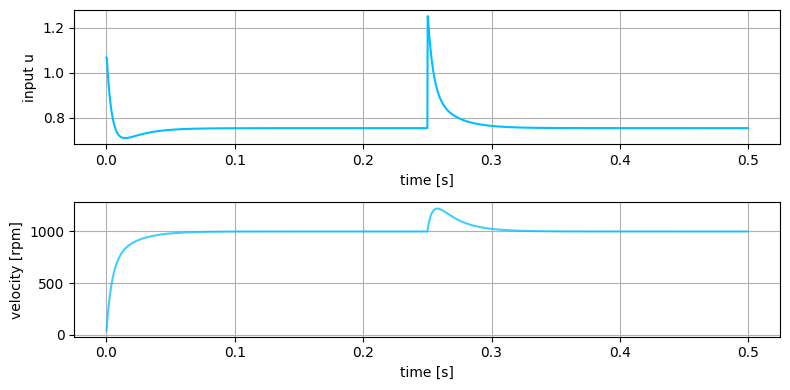
\includegraphics[scale=0.8]{../images/motor_control/pid_pi_control_1.png}
                    \caption{PI controller with correct parameters}
                    \label{fig:pi_controller_correct}
                \end{figure}
                
            \newpage
            \subsection{complete discrete PID algorithm}  
    
                \begin{enumerate}
                  \item  calculate u-change candidate :
                    $$\Delta \hat{u}(n) = k_0e(n) + k_1e(n) + k_2e(n)$$
                  
                  \item clip maximum allowed u-change, to avoid u-kick :
                    $$\Delta u(n) = clip(\Delta \hat{u}(n), -du_{min}, du_{max})$$
              
                  \item clip maximum allowed u value, to avoid saturation / windup :
                    $$u(n) = clip(u(n-1) + \Delta u(n), -u_{min}, u_{max})$$
                \end{enumerate}

                Full Python code example for discrete PID controller :
                \begin{lstlisting}[style=python_style]
class PID:

def __init__(self, kp, ki, kd, antiwindup = 10**10, du_max=10**10):
    self.k0 = kp + ki + kd
    self.k1 = -kp -2.0*kd
    self.k2 = kd

    self.e0 = 0.0
    self.e1 = 0.0
    self.e2 = 0.0
    
    self.antiwindup = antiwindup
    self.du_max     = du_max

def forward(self, xr, x, u_prev):
    # error compute
    self.e2 = self.e1
    self.e1 = self.e0
    self.e0 = xr - x

    # u-change computing
    du = self.k0*self.e0 + self.k1*self.e1 + self.k2*self.e2

    # kick clipping, maximum output value change limitation
    du  = numpy.clip(du, -self.du_max , self.du_max)

    # antiwindup, maximum output value limitation
    u   = numpy.clip(u_prev + du,  -self.antiwindup, self.antiwindup)

    return u


                \end{lstlisting}


    \newpage
    \section{Optimal control}

                
        Optimal control is solution of following optimisation problem

        \begin{align}
            \min_{x(.), u(.)} \sum_{n=0}^\infty x^T(n)Qx(n) + u^T(n)Ru(n) \\
            s.t.\ x(n+1) = Ax(n) + Bu(n)
        \end{align}

        the cost function is quadratic
        \begin{align}
            J &= \sum_{n=0}^\infty x^T(n)Qx(n) + u^T(n)Ru(n)
        \end{align}

        where $Q$ and $R$ are positive semidefinite square matrices, with shapes $N \times N$ and $M \times M$ respectively.
        The system order is $N$ and system have $M$ inputs.
        Matrix $Q$ penalises magnitude of $x(n)$ elements, matrix $R$ penalises control input $u(n)$ elements.
        Solution is obtained by solving algebraic Riccati equation, and results in feedback gain $u(n) = -Kx(n)$.
        This controller is called \textbf{Linear Quadratic Regulator - LQR}.
        This matrix can fully manipulate with system poles and guarantee system stability.
        However, given structure have steady state error - brings system always into zero state.
        To eliminate this issue, we introduce integral action term by augmenting system matrices. 
        Resulted controller have two matrices : feedback gain $K$ and integral action gain $K_i$ matrix.
        The modified LQR controller have form on following fig \ref{fig:control_lqr_generic} 
        with equations \ref{eq:lqr_integral_action}.

        \begin{figure}[!htb]
            \centering
            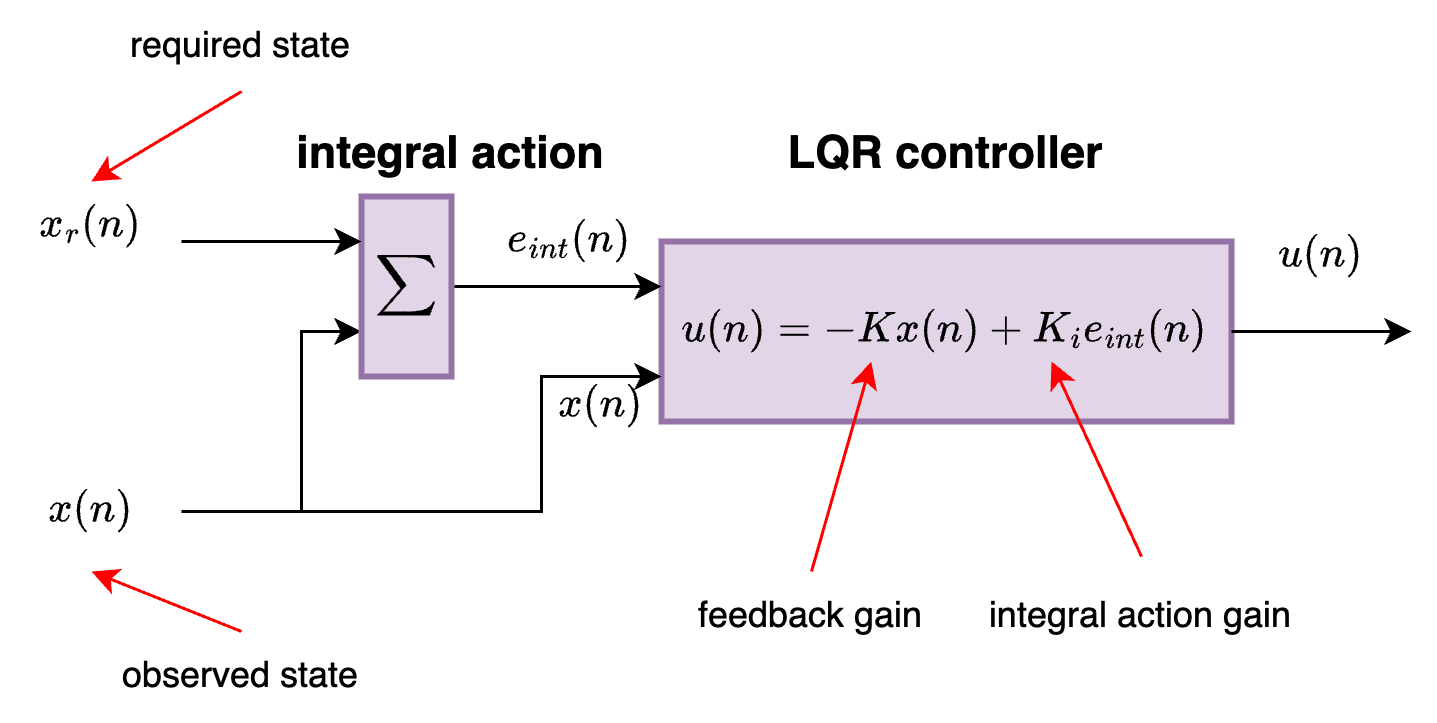
\includegraphics[scale=0.8]{../diagrams/control_generic/control_generic-lqr_discrete.png}
            \caption{LQR controller with integral action}
            \label{fig:control_lqr_generic}
        \end{figure}

        \begin{align}
            u(n)&= -Kx(n) + K_ie_{int}(n) \label{eq:lqr_integral_action} \\
            e_{int}(n)& = e_{int}(n-1) + x_r(n) - x(n)
        \end{align}

        where : 
        \begin{itemize}
            \item $x(n)$ is observerd state, column vector, with shape $(N, 1)$
            \item $x_r(n)$ is required state, column vector, with shape $(N, 1)$
            \item $u(n)$ is controller output, column vector, with shape $(M, 1)$
            \item $K$ is feedback gain matrix, with shape $(M, N)$
            \item $K_i$ is integral gain matrix, with shape $(M, N)$ 
        \end{itemize}


        \begin{figure}[!htb]
            \centering
            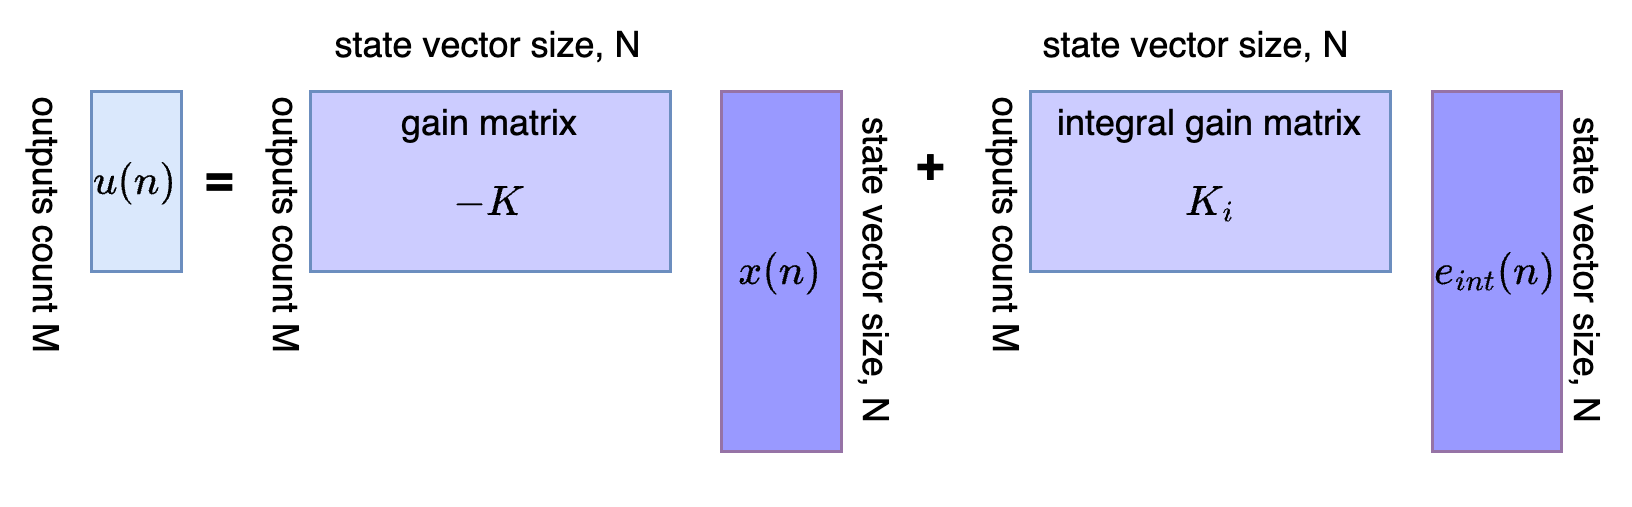
\includegraphics[scale=0.8]{../diagrams/control_generic/control_generic-lqr_detail.png}
            \caption{Matrices shapes in LQR controller}
            \label{fig:control_lqr_matrices_shape}
        \end{figure}
        


\end{document}